\documentclass[../main.tex]{subfiles}

\begin{document}

\section{Projektplanlægning}

%Indledning af projekt-afsnittet
\subsection{Udviklingsproces for forløb}
\begin{flushleft}
\todo [Skal have mindre omskrivninger - se evt. CDIO2] \newline
   For dette projekt har vi primært haft den samme strategi for udarbejdelse af projektet, som i CDIO-2. Her har vi taget udgangspunkt i Unified Proces (UP), som vores udvilkingsproces. Som nævnt i indledningen dækker UP over at opdele projektet i mindre delelementer, kaldet iterationer. Disse iterationer bliver samlet løbende, hvilket kaldes at projektet vil vokse iterativt - altså at projeketet vokser stødt, efter hver fuldførte delelement. UP kan stilles op i en model, som viser de forskellige faser, descipliner og iterationer for UP-projekt:
\end{flushleft}

%UP-model
\begin{figure}[H]
    \begin{center}
   {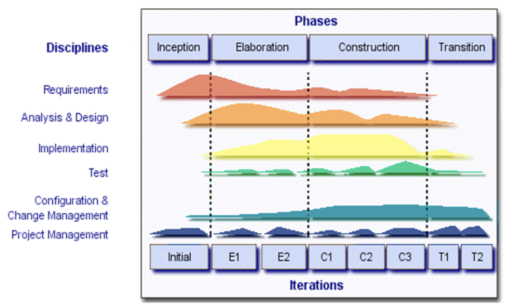
\includegraphics[width=0.45\textheight]{figures/UP-model.png}}
    \caption{UP forløb. \cite{UPModel} }
    
    \end{center}
\end{figure}



%Beskrivelse af vores projektplanlægning
\subsection{Planlagte forløb}
\begin{flushleft}
Vi har ligesom i CDIO-2 valgt at sætte os ned samlet, for at få fastsat datoer for, hvornår vi ønskede hver fase af projektet ville ønskes færdigt.

   - Krav og analyse lavet sammen (først) \newline
   - Designklassedigram gennemgået sammen \newline
   - Lært fra sidst -> noget kode skal være færdigt før andre.\newline
   > alle har en idé om hvad der skal laves.\newline
  
   Deadlines: \newline
   - Analyse og krav  6/11 \newline
   - Design 7/11\newline
   - Kode (første runde) d. 13/11\newline %nok færdig omkring d. 20/11.
   - Kode (anden runde) d. 18/11\newline
   - Rapport 25/11\newline
   
   - gantt kort ofc.
   
\end{flushleft}

%Beskr (andenivelser af faktiske forløb.
\subsection{Faktiske forløb}
\begin{flushleft}
   - Inddraget metoder vi ikke har lært i undervisningen -> XML og ArrayList -> ikke nødvendigt \newline
   - Mere tid i Design (designklassediagram) -> Ikke præcise nok i hvad der faktisk skal laves, mere bare en overordnet retningslinje. \newline
   - Inddraget Deck klasse senere (ca. den 16.) -> i sammenhængen med forrige punkt. \newline
   - Daniel(Kunde) har svaret senere på spørgsmål med vilje -> bare godt at have med. \newline
   - Ikke taget højde for andre opgaver/afleveringer. \newline
\end{flushleft}

\todo Måske skrive at vi har haft kontakt med kunden, som en del af vores projektplanglægning

\end{document}